\chapter{Prototype Implementation}
\label{chapter:implementation}

For the implementation of contracting service, I have used Django framework, because it is powerful, but also easy to use, and it provides a fixed structure to organize the project. Django framework provides built-in modules for most of the common functionalities with a good security architecture. Along with Django, I have used Bootstrap for styling since it is light-weight and simple.

In this chapter, I will present a brief description of technologies that I used followed by a brief overview of the whole project, showing how different parts fit together before digging into details.

\section{Technologies Used}
\label{section:technologiesUsed}

In the following text, I will describe two technologies that were used for this implementation in order to give justification of why they are a perfect fit for this project.

\subsection{Django Framework}

Django is a high-level Python Web framework that unlike a library, forces a structure to separate concerns and encourage rapid development and clean, pragmatic design. Structure of Django is influenced by Model-view-controller (MVC), which is a pattern used in software architecture for interactive software or application. 

Model maintains the state of the application by holding the data. In web development, that data is stored in a database. Model abstracts the database typically using a Object-relational-mapper (OBM),	 which maps the data to objects (in case of Django, python objects) and vice versa. Model also takes care of any restrictions on data and takes care of validating, making sure that correct data is stored.

Concern of the view is to generate user interface. In web applications, this means producing HTML typically using a \emph{templating language}. Data is acquired from the Model (typically through Controller, which will be explained in further text) and mixed with HTML using templating language. View can format the data to suit the requirements of a particular view. In simple words, view controls what user sees.

Controller, in a simplest interpretation, controls which views to use based on user input and data from the models. In a broader interpretation, it handles business logic, using models and what rules they enforce.

Django Framework uses a variation on the traditional MVC pattern called Model-Template-View (MTV). Firstly, role of the Model is the same as in MVC, where Django abstracts the database using OBM, instead of tables you deal with classes and instances of data as objects. Secondly, the role of View in MVC is represented in Django using Templates and View. View in Django has a slightly different meaning than in MVC. It represents, which data needs to be presented to a user, not necessarily how the data looks. Views get user input (HTTP request), then they access necessary models followed by processing of data, if necessary, and pass it to Templates. Role of Templates is to create the final HTML presented to a user using the data from Views. Finally, role of the Controller can be viewed as whole framework and URL-routing. URL-routing is achieved in Django with a simple 'urls.py' file, which links URLs to views.

Django Framework provides built-in solutions for most of the common tasks that almost every website has. Since this work is not about Django Framework I will only cite subset of parts used in this prototype:

\begin{enumerate}
	\setlength{\itemsep}{1pt}
	\item \textbf{\textit{User management}}: including creating users, authenticating users, creating sessions, managing cookies, managing user groups and more.
	\item \textbf{\textit{Security mechanisms}}: in order to prevent most common forms of cyberattacks such is cross-site request forgery.
	\item \textbf{\textit{Support for number of email back-ends}}.
	\item \textbf{\textit{Efficient mechanism for creating forms from Models}}.
	\item \textbf{\textit{Creating custom decorators to provide authorization for certain groups of users to a view}}.
\end{enumerate}

Most importantly, Django Framework has an enormous user base and excellent documentation making it very comfortable to work with. Having a big user base means that most of the questions you might have are already answered and easily accessible. These are the reasons I have chosen Django for this so lution.

\subsection{Bootstrap}

Bootstrap is an open source toolkit for developing with HTML, CSS, and JS. It is very light weight and perfect for applications that do not require a lot of styling. Bootstrap library is easily included in Django templates using just a \verb!<link>! HTML tag.

Bootstrap library is only one CSS file providing many different classes for styling appealing to human visual cues (for example, red for danger, blue for default and more). It relies on a twelve column system for layout, which, if used correctly, brings responsiveness (for different screen sized) on its own. Bootstrap has a big community of users who share snippets of their code providing different functionalities fulfilling almost any need in modern web development.

\section{Overview}

This solution is a Web platform for managing small devices and controlling who has access to the data they generate. Most challenging part was understanding the users of the platform and their needs. Following section describes account types, which correspond to roles they have, followed by the brief description of main parts of the platform.

\subsection{Account Types}

In the Industrial Internet context, I have identified four different types of accounts, with their separate views of the platform depending on their role. Views of these accounts have a common core although they are suited for different purposes. 

Firstly, there needs to be a central authority that distributes accounts to verified manufacturers of industrial machines. In order to receive manufacturer account you need to contact this central authority, which could be a standardization agency but it can be any impartial actor. When that authority verifies that your company is who they claim to be, several accounts can be issued depending on the number of departments that company has or any other criteria depending on the agreement with the manufacturer company. Since the only responsibility this authority has is creating accounts for manufacturers I have used standard Django admin page (and admin account) for its implementation, stripped down to only basic functionality for managing accounts.

Secondly, manufacturers account is assigned to companies that produce smart machines. Their responsibility is to add devices (and update their information if necessary) to platform and assign them to machines (detailed description of devices will be given in subsection \ref{deviceManagement}), which are abstract representation of real machine (such is a smart crane) and devices it possess. When the machine has been bought by the customer, manufacturer creates an account for customer (in case they do not possess one) and assigns it to them, giving them full control over who can communicate with that machine. In a case where a customer already has an account, it is customers responsibility to ``subscribe'' to manufacturer in order for manufacturer to see their account, this is done through a simple form, which will be described in section \ref{section:customer}. Manufacturer account will be described in detail in section \ref{Manufacturer}.

Thirdly, customer account is assigned to owners of the smart machines. Their view is restricted to only devices and machines that they possess and they can manage policies (control access to devices) for those devices only. Along with the possibility of managing policies, customer account can create multiple user accounts (which represents people responsible for single machines or group of them) and assign machines or devices to them. In this way, customer account has a full overview of what policies are in place and who created them while also being able to add or remove faulty ones or general ones (like allowing customers work computer to access all the data or opening their data to a statistical agency). By being able to create user accounts customer can pass on the responsibility and fine tuning of policies for certain machines down the hierarchy of the company.

Finally, user account is assigned to people responsible for a subset of machines that a customer company possess. These accounts are restricted to only managing policies of the machines assigned to them without the possibility to create more accounts or manage devices in the system. Overview of accounts and their views are visualized in figure \ref{fig:accountTypes}.

\begin{figure}[ht]
	\begin{center}
		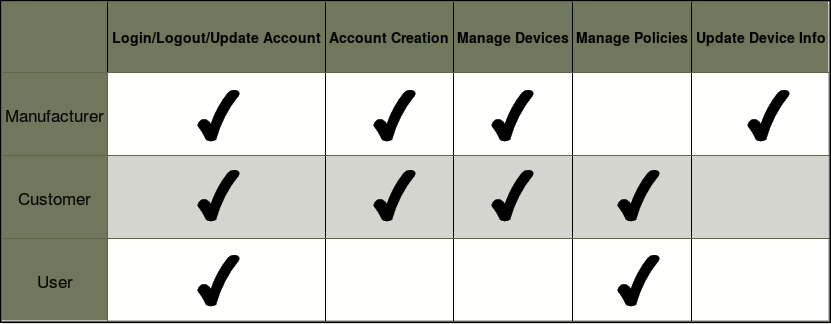
\includegraphics[width=\textwidth]{images/Functionalities}
		\caption{Account types and their views}
		\label{fig:accountTypes}
	\end{center}
\end{figure}

\subsection{Device Management}
\label{deviceManagement}

As previously mentioned, manufacturers task is to add devices to the system, filling all necessary information about the device defined by LWM2M standard described in \ref{section:LWM2M}. This information consists of manufacturer name, model number, serial number, public key or identity of the device along with a descriptive name used to refer to it in the system. Public key or identity according to LWM2M standard could be a certificate, a pre-shared key, raw public key or nothing. Since all these, except last one, are similar and exist in standard only to provide flexibility for the manufacturers, only pre-shared key is supported in this solution, although it can easily be extended. 

Further following LWM2M standard, which has a client-server architecture, devices act as a client where my solution acts as a bootstrap server. When a device gets connected to a network, it communicates its IP address (in a form of IPv4 or IPv6) and FQDN or MSISDN to a bootstrap server which saves it for use when managing policies. Example of information implanted on a device is shown on figure \ref{fig:device}.

\begin{figure}[ht]
	\begin{center}
		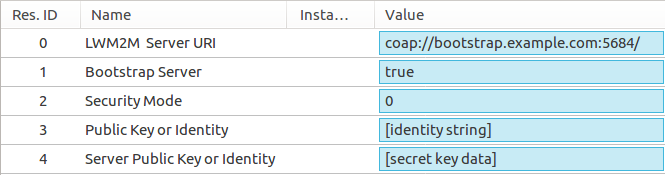
\includegraphics[width=\textwidth]{images/Device}
		\caption{Example device}
		\label{fig:device}
	\end{center}
\end{figure}

Server URI represents the URI of my server, which enables a device to locate it. Only after the server has verified identity of the device, using pre-shared key, it can store devices IP address. In an event when a device is moved to another network (changing its IP address), a device communicates a new IP address, which replaces the old one and all policies get updated with a new address.

\subsection{Policy Management}
\label{policyManagement}

Work described in section \ref{CES} is very extensive and is made with mobile communications in mind. Although, the idea of policy based communications is perfectly suitable for these purposes since allowing communication between a device and some host can be done in one simple HTTP request to Policy Database. Policy Database holds all policies describing who is allowed to communicate with whom. This database could be distributed or in one central place, although that is outside of the scope of this work, but it has one API that hides the way database is arranged and is the only way database can be accessed. 

Only four different API requests are used in this work. These requests are for inserting, deleting, retrieving and updating firewall policies using Http Post for inserting and deleting, Http get for retrieving and Http put for updating. Inserting policies require following information and they are sufficient for the CES node to determine whether the communication should be established, whether the package should be dropped at the edge: 

\begin{enumerate}
	\setlength{\itemsep}{1pt}
	\item \textbf{\textit{Target IP address and port}}: target represents a host wanting to communicate with a device.
	\item \textbf{\textit{Source IP address and port}}: representing a device, extracted from a database in my system.
	\item \textbf{\textit{Start and end of validity timestamps}}: allowing scheduling of access to devices.
	\item \textbf{\textit{Direction of communication}}: representing, whether only reporting of data from the device to the host is allowed, sending data to a device or both.
	\item \textbf{\textit{Transport protocol}}: in this case CoAP is used, justification is provided in section \ref{section:LWM2M}.
	\item \textbf{\textit{FQDN or MSISDN}}: helps speed up the search for receivers as mentioned in section \ref{CES} and is used for querying policies.
\end{enumerate}

Direction of communication can be bi-directional or uni-directional (from host to device, or device to host). Bi-directional communication is a regular case, when a host sends a request to a device and gets data or acknowledgment in return. Uni-directional communication is useful in cases where the devices just need to send data (for example, temperature readings) to some external host who is subscribed to them, without a possibility of that host controlling the device (for example, sending request for shutdown). Other way around, uni-directional communication from host to a device could be useful in rare cases where a host is allowed to request from a device to do a task, or send data to some other host. Therefore, all three options are supported in this work.

Deleting and retrieving policies is done using only FQDN or MSISDN (depending on, which one is available for a device), where updating is done the same way as for inserting only different HTTP verb is used. Graphical interface for managing policies will be described in the remainder of this section where all views from different accounts are explained.

\section{Manufacturer}
\label{Manufacturer}

When manufacturer creates session by logging-in to the platform he is directed to a home page. Home page for manufacturers contains (along with navigation bar, which is always present) only a simple form to create customer account pictured on figure \ref{fig:CreateCustomer}. This form, along with most of the forms in this solution, is created using Django ModelForm, which created a form using database model of a user. When the form is submitted, customer account is made inactive and an automatic email is sent to the provided email address for verification. Automated emails are realized in this prototype using django built-in wrapper for python smtplib module, using a google email account. Only after the customer follows the link in the email, their account is made active and they are prompted to change their password and provide additional information using update form pictured on figure \ref{fig:UpdateAccount}. Update account form is available to all types of accounts, to encourage password change in order to promote security.

%TODO: Merge these two in one
\begin{figure}
	\begin{center}
		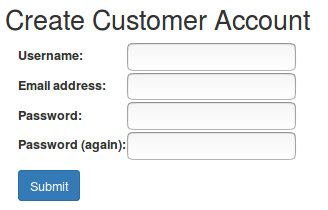
\includegraphics[width=0.4\textwidth]{images/implementation/CreateCustomer}
		\caption{Create Customer}
		\label{fig:CreateCustomer}
	\end{center}
\end{figure}

\begin{figure}[ht]
	\begin{center}
		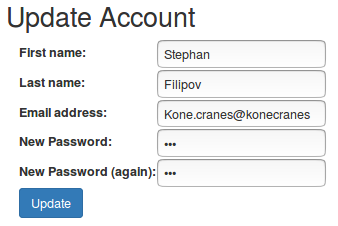
\includegraphics[width=0.4\textwidth]{images/implementation/UpdateAccount}
		\caption{Update Account}
		\label{fig:UpdateAccount}
	\end{center}
\end{figure}

As previously mentioned, manufacturers task is to add devices to platform, which they can later assign to customers that have bought them. Adding of devices is made available in two ways: through ``Manage Devices'' page for custom made machines, or following a previously defined template. For the custom machines, first a machine needs to be created. Machine is an abstract concept that only has a name, which is used to organize devices. For example, AaltoCrane could be a machine and all sensors and actuators that are mounted on that crane are assigned to it. In the process of adding a device to the platform, a machine it belongs to needs to be specified. Note that in order to remove a machine from platform, its name needs to be typed in the text box to prevent accidental removal of machines. Two forms needed to complete this task are pictured on figure \ref{fig:AddMachineDevice}. 

\begin{figure}[ht]
	\begin{center}
		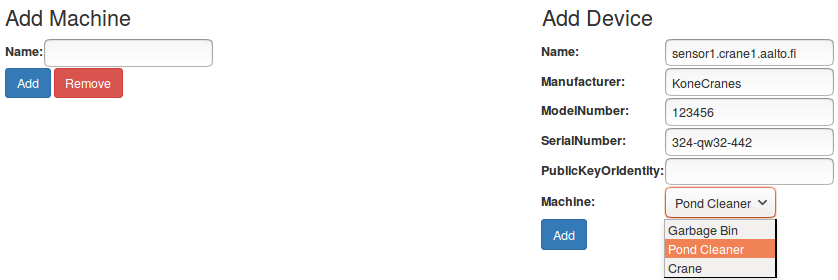
\includegraphics[width=\textwidth]{images/implementation/AddMachineDevice}
		\caption{Adding machines and devices}
		\label{fig:AddMachineDevice}
	\end{center}
\end{figure}

% Mention how templates can be extended in evaluation or future work discussion(mention digital twin)
Other way a manufacturer adds devices is through templates. Templates define how many devices a particular machine that a manufacturer produces has so that when a new machine is created, template can be instantiated to add a new machine. Creation and overview of templates is pictured on figure \ref{fig:addTemplate}. 

\begin{figure}[ht]
	\begin{center}
		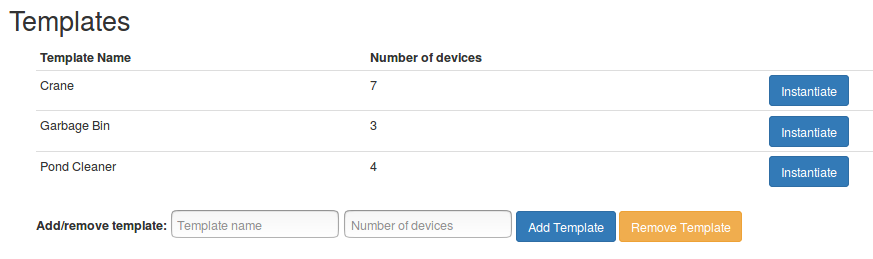
\includegraphics[width=\textwidth]{images/implementation/AddTemplate}
		\caption{Creation and overview of Templates}
		\label{fig:addTemplate}
	\end{center}
\end{figure}

Clicking on the ``instantiate'' button for a particular machine opens a form bellow. This form asks for the name of the machine (which is supposed to be descriptive, for example Aalto Industrial Campus Crane or similar), and information about devices attached to it. Number of devices in a form is equal to the number defined in the template. Form for a machine with three devices is pictured on figure \ref{fig:AddMachineViaTemplate}.

\begin{figure}[ht]
	\begin{center}
		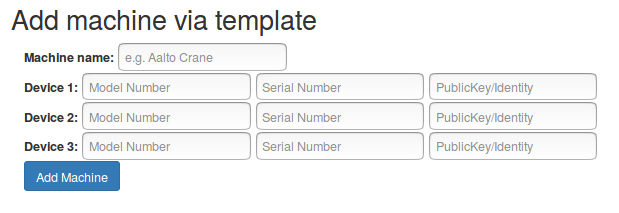
\includegraphics[width=\textwidth]{images/implementation/AddMachineViaTemplate}
		\caption{Instantiating a template with three devices}
		\label{fig:AddMachineViaTemplate}
	\end{center}
\end{figure}

When the customer has an account and all devices are added to the platform and organized to machines, manufacturer needs to assign these devices to customers. Assigning devices to customers can be done on a device level or machine level as pictured on figure \ref{fig:ManageDevicesCompany}. No matter if the manufacturer is assigning devices or machines (group of devices) the task is done through a simple form and clicking on an appropriate button, either to add or remove a customer. Removing a customer makes sense in case when a machine or device has been rented or a mistake was made while adding. Removing of devices from a platform is also in a same view because it provides a good overview of which devices are attached to which machines.

\begin{figure}[ht]
	\begin{center}
		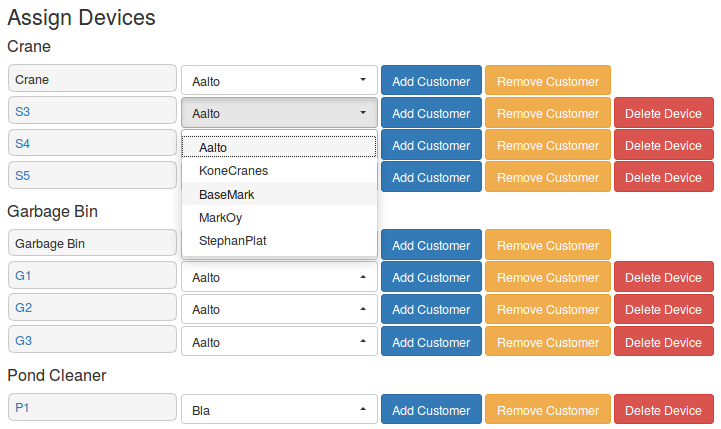
\includegraphics[width=\textwidth]{images/implementation/ManageDevicesCompany}
		\caption{Device Management For Manufacturer}
		\label{fig:ManageDevicesCompany}
	\end{center}
\end{figure}	

In the figure \ref{fig:ManageDevicesCompany}, clicking on a device name navigates to a separate page where details about a device can be inspected, and changed if needed as pictured on figure \ref{fig:DeviceDetailsUpdate}. Fields in the form are pre-filled with current information about a device, so that typing mistakes or any small changes can be made easily.

\begin{figure}[ht]
	\begin{center}
		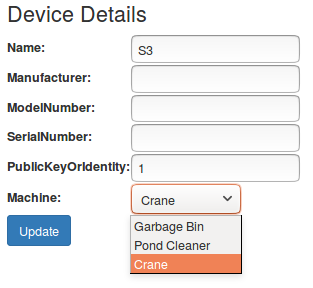
\includegraphics[width=0.4\textwidth]{images/implementation/DeviceDetailsUpdate}
		\caption{Update Device Information}
		\label{fig:DeviceDetailsUpdate}
	\end{center}
\end{figure}

Last element on a Manage Devices page is pictured on figure \ref{fig:DeviceAssignment}. This element only provides an overview of which users are assigned to which devices. It is intended to be used along with element pictured on figure \ref{fig:ManageDevicesCompany} in order to check, whether any mistakes were made and that everything is how it should be.

\begin{figure}[ht]
	\begin{center}
		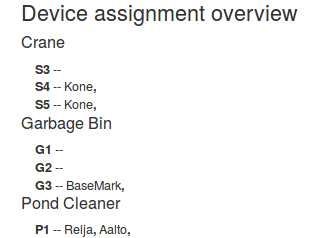
\includegraphics[width=0.4\textwidth]{images/implementation/DeviceAssignment}
		\caption{Device Assignment Overview}
		\label{fig:DeviceAssignment}
	\end{center}
\end{figure}


\section{Customer}
\label{section:customer}

 After logging-in to the platform, customer is directed to a home page where he can create additional user accounts. Creation of user accounts is slightly different from customer accounts as pictured on figure \ref{fig:CreateUser}. In the form, for convenience sake, customer can assign devices to a user while creating the account using a multiple choice select field. In case when the account is created for just one device or a small set of devices, this can greatly reduce the number of clicks and queries to the database to complete a task. As with customer accounts, user accounts also need email verification.

\begin{figure}[ht]
	\begin{center}
		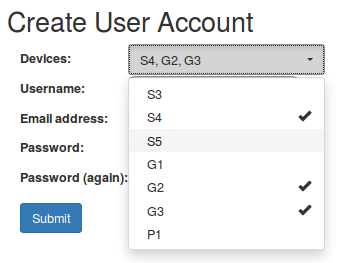
\includegraphics[width=0.6\textwidth]{images/implementation/CreateUser}
		\caption{User Account Creation}
		\label{fig:CreateUser}
	\end{center}
\end{figure}

One very simple but necessary element pictured on figure \ref{fig:SubscribeToManufacturer} allows a customer to subscribe to the manufacturer and in that way be visible to manufacturer when assigning devices. Customer only needs to type the name of the manufacturer (that manufacturer communicated to customer in the process of buying the machine) and submit.

\begin{figure}[ht]
	\begin{center}
		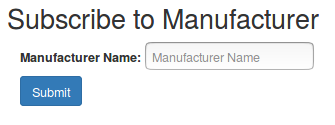
\includegraphics[width=0.6\textwidth]{images/implementation/SubscribeToManufacturer}
		\caption{Inform Manufacturer that you are a customer}
		\label{fig:SubscribeToManufacturer}
	\end{center}
\end{figure}

On ``Device Management'' page, customer can assign devices to users. His view is restricted only to devices that are previously assigned to him by the manufacturer, and choice of users is restricted to the ones he created (which represent users he is responsible for). Interface for doing this resembles one pictured in figure \ref{fig:ManageDevicesCompany} with two exceptions: customer is not allowed to change details about devices; and user is not allowed to 
delete devices from the system. In the case when a machine is no longer used (not needed anymore or replaced with a new one), manufacturer needs to be contacted directly in order to remove the machine from platform. This is because customers can not be allowed to add devices, and if they were allowed to remove devices, they could mistakenly remove the device without the possibility of adding it back. In industrial case, these machines are expensive, large and robust, therefore, they do not need to be removed frequently, which is why I opted for this solution.

As previously mentioned, only customers and users are allowed to control who can communicate with their devices and they control that through policies. ``Manage Policies'' page contains two elements, one for adding policies, other for removing them and to give overview of existing ones. Customer view is restricted to only devices that are assigned to him (as in case of managing devices) and he can add policies to Policy database using a group of forms pictured on figure \ref{fig:ManagePolicies}. Customer only needs to specify IP address (both IPv4 and IPv6 supported) of a host, direction of communication (as explained in \ref{policyManagement}), start and end date of policy validity, and click on submit policy. By submitting a policy, customer has allowed a host with specified IP address to interact with a device or all devices that are part of a machine.

\begin{figure}[ht]
	\begin{center}
		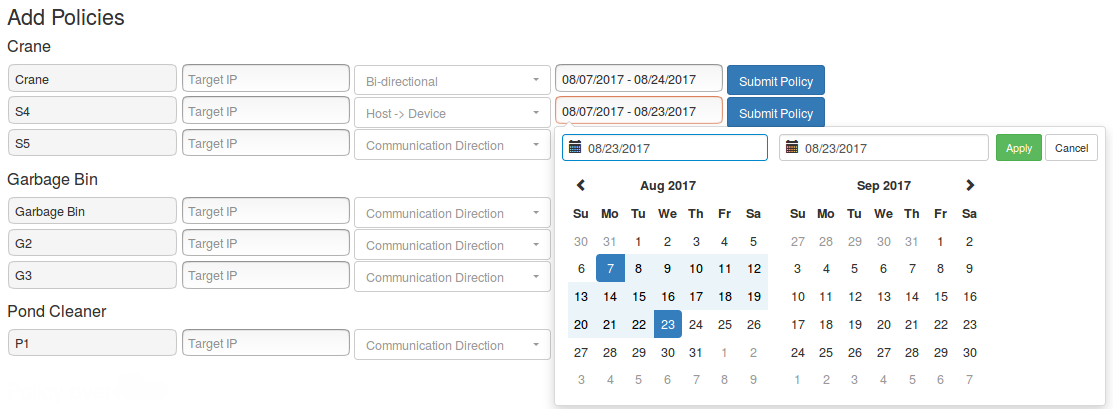
\includegraphics[width=\textwidth]{images/implementation/ManagePolicies}
		\caption{Policy Management}
		\label{fig:ManagePolicies}
	\end{center}
\end{figure}

Second element on a ``Manage Policies'' page contains overview of all policies related to devices that a customer has. In the same element, customer can remove policies that are mistakenly made or if the circumstances changed since the policy was put in place.

\begin{figure}[ht]
	\begin{center}
		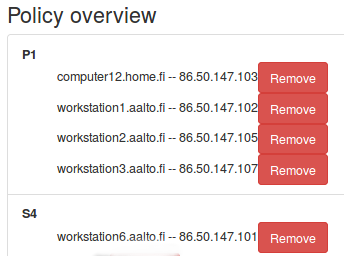
\includegraphics[width=0.6\textwidth]{images/implementation/PolicyOverview}
		\caption{Overview of policies}
		\label{fig:PolicyOverview}
	\end{center}
\end{figure}

\section{User}

Simplest account type is user account. User account can only update information about his account and manage policies for the devices he was assigned to by the customer. ``Manage Policies'' page for user only contains elements pictured in figures \ref{fig:ManagePolicies} and \ref{fig:PolicyOverview}.




